\documentclass{article}
\usepackage{amssymb}
\usepackage{amsmath}
\usepackage{mathtools}
\usepackage{centernot}
\usepackage{algpseudocode}
\usepackage{graphicx}
\usepackage[margin=1in]{geometry}
\setlength{\parindent}{0in}

\begin{document}

\title{EE360C: Lab 1}
\author{Joshua Dong (jid295)}
\date{\today}
\maketitle

\section*{1. Algorithm Analysis}
\subsection*{a) bounds}
The runtime is $O(n^3)$. The outer loop loops in quadratic time. Adding the
entries from $A[i]$ to $A[j]$ is bounded above by n. Since
$\left|j - i\right|$ is dominated by n, adding the entries is also bounded
below by a factor of n. Then we can conclude that the runtime is
$\Theta(n^3)$.

\subsection*{b) algorithm}
Since we recompute so many values, we could clearly be more
efficient by using a memoization approach. For example:
\begin{algorithmic}
\For {$i \gets 1..n$}
    \For {$j \gets i+1..n$}
        \If {$j = i+1$}
            \State {$B[i,j] = A[i] + A[j]$}
        \Else
            \State {$B[i,j] = B[i,j-1] + A[j]$}
        \EndIf
    \EndFor
\EndFor
\end{algorithmic}

\subsection*{c) runtime}
The runtime is $O(n^2)$ since we still loop over a quadratic number of
elements, but we do not require $O(n)$ for each iteration of the loop.


\newpage
\section*{2. Decision Trees}
\subsection*{a) heavy ball}
Trinary search would find the ball in two rounds: first weigh two thirds
of the balls, one third on each side. If they are equal, then repeat the
algorithm with the unweighed group. If they are not equal, then repeat the
algorithm with the heavier group.

\subsection*{b) decision tree}
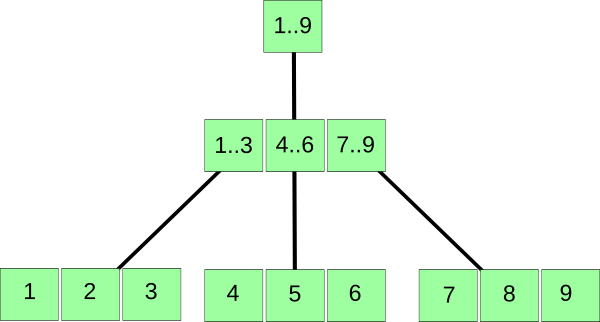
\includegraphics[width=240px]{graphs/tree.png}


\section*{3. Heap}
Suppose we implement a breadth-first search:
\begin{algorithmic}
\State {$Results \coloneqq$ empty list}
\State {$Queue \coloneqq$ empty queue}
\State {$Queue \gets$ root}
\While {$Queue$ not empty}
    \State {$Current \gets Queue$}
    \For {$Child \in$ children of $Current$}
        \If {$Child \leq$ VALUE}
            \State {$Results \gets Child$}
            \State {$Queue \gets Child$}
        \EndIf
    \EndFor
\EndWhile
\end{algorithmic}
Then our time complexity would be $O(n)$, where $n$ is the number of elements
in the heap.


\newpage
\section*{4. Graphs}
\subsection*{a) counterexample}

\includegraphics{graphs/4a.png}
\subsection*{b) counterexample}
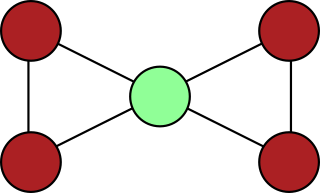
\includegraphics{graphs/4b.png}


\section*{5. Graphs}
$T$ never produces a cyclic graph, because trees by definition have no cycles.
If $G$ is cyclic, then $T$ cannot be equal to $G$ since a cyclic graph cannot
have the same edges as an acyclic graph. Then we have shown that if a $G$ is
cyclic, then the depth-first and breadth-first tree generated from a node $u$
in $G$ differs from $G$. The contrapositive of this statement is that if the
depth-first search tree is the same as the breadth-first search tree for a
graph $G$, then $G$ is acyclic.
\\\\
Suppose $T$ is both a depth-first search tree and a breadth-first search tree
rooted at $u$ of a connected graph $G$. Then $G$ is acyclic. Since $G$ is
connected, $T$ has every vertex of $G$. Suppose $G$ has an edge $e$ not
contained in $T$. By definition of a finite tree, adding an edge to $T$
would create a cycle. But $G$ is acyclic, so $e$ is not in $G$, contradiction.
Then no edge in $G$ is not in $T$, which is what we sought to prove.

\end{document}
